

\section{Dispositivos Lógico Programáveis}
	\begin{frame}{Dispositivos Lógico Programáveis}
		\begin{figure}[H]
			\centering
			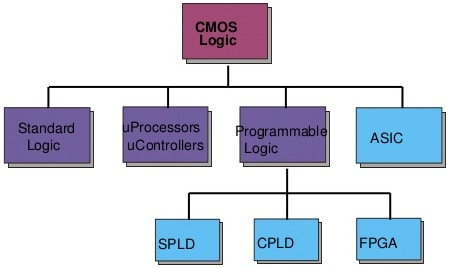
\includegraphics[width=0.8\textwidth]{img/intro/arvore.jpg}
			\caption{ASIC vs. PLD.}
		\end{figure}
	\end{frame}

	\begin{frame}{Dispositivos Lógico Programáveis}
		\begin{figure}[H]
			\centering
			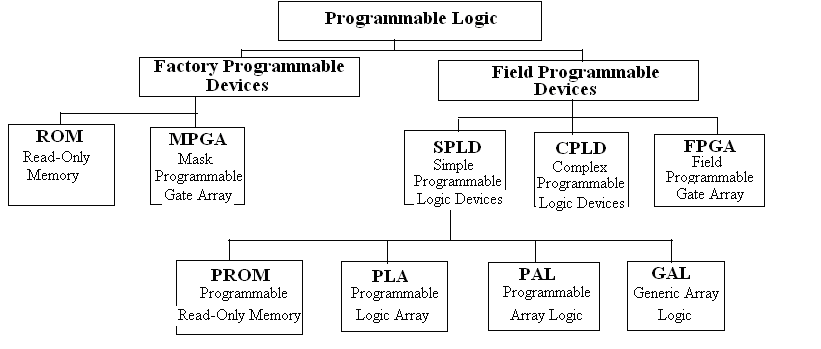
\includegraphics[width=1.0\textwidth]{img/intro/arvore-pld.png}
			\caption{\textit{Programmable Logic Device}.}
		\end{figure}
	\end{frame}

	\begin{frame}{Dispositivos Lógico Programáveis}
		\begin{itemize}
			\setlength\itemsep{1.4em}

			\item Tocci \cite{Tocci2003} cita que os dispositivos lógicos programáveis (PLD\footnote{do inglês \textit{Programmable Logic Device}.}) são as ``\textit{maravilhas de flexibilidade de projeto}''.

			\item Ao contrário de uma porta lógica, que tem uma função fixa, um PLD tem uma função indefinida após a sua fabricação.

			\item Para utilizá-lo em um circuito, deve-se \textbf{programá-lo previamente}.

			\item A lógica programável proporciona ao projetista:
			\begin{itemize}
				\setlength\itemsep{0.5em}
				\item A possibilidade de se \textbf{adequar aos vários níveis de projetos} sendo estes:
				\begin{itemize}
					\item Para desenvolvimento de protótipos ou mesmo circuitos finais.
				\end{itemize}

				\item \textbf{Fácil alteração} do projeto a \textbf{qualquer momento};

				\item Programação por meio de Álgebra Boole, Mapa de Karnaugh, e Linguagens de Descrição de \textit{Hardware}.
			\end{itemize}
		\end{itemize}
	\end{frame}

	\begin{frame}{Dispositivos Lógico Programáveis}
		\begin{figure}[H]
			\centering
			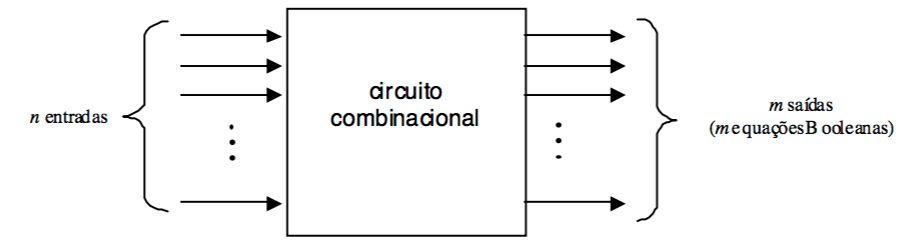
\includegraphics[width=1\textwidth]{img/fpga/geral1.png}
			\caption{Exemplo de um circuito combinacional.}
		\end{figure}
	\end{frame}

	\begin{frame}{Dispositivos Lógico Programáveis - FPGA}
		\begin{itemize}
			\setlength\itemsep{1.4em}

			\item Em meados dos anos 80, a empresa \textbf{Xilinx} e Gerald Estrin anuncia uma nova arquitetura.

			\begin{itemize}\setlength\itemsep{0.4em}
				\item Isso foi um \textbf{choque} na época pois cria-se então um \textbf{novo paradigma de projetos de circuitos integrados};

				\item Entre vários tipos de PLD existe um tipo que é baseado na tecnologia \textit{gate array} e é chamado de FPGA\footnote{Do inglês \textit{Field-Programmable Gate Array}, Arranjo de Portas Programável em Campo.}.
			\end{itemize}


			\item O FPGA usa uma rede de portas lógicas cuja programação é feita pelo \textbf{projetista e não pelo fabricante}.
			\begin{itemize}
				\item Sendo reprogramados, o usuário pode utilizá-lo num projeto e logo em seguida reprogramá-lo para que execute outro projeto.
			\end{itemize}

			\item Deixando mais claro, o termo ``\textbf{campo}'' na nomenclatura é apenas um termo da engenharia utilizado para indicar o \textbf{mundo de fora da fábrica}.
		\end{itemize}
	\end{frame}

	\begin{frame}{Dispositivos Lógico Programáveis - FPGA}
		\begin{itemize}
			\setlength\itemsep{1.6em}

			\item Excelentes para \textbf{desenvolver um protótipo de circuito integrado} a fim da realização de testes \textbf{antes da fabricação em massa} \cite{Skliarova2003} e \textbf{ensino}.

			\item Seu custo em relação ao ASIC\footnote{Do inglês \textit{Application Specific Integrated Circuits}.} é menor;

			\item Seu tempo total gasto desde a especificação do projeto até sua sintetização também é menor
			\begin{itemize}
				\setlength\itemsep{0.5em}

				\item ASICs são produzidos geralmente em \textbf{larga} escala
				\begin{itemize}
					\item O custo de fabricação de 1 circuito é caro;
					\item O custo de fabricação em massa também é caro.
				\end{itemize}

				\item Qualquer erro no ASIC, deve-se reiniciar todo o processo de desenvolvimento
				\begin{itemize}
					\item Sendo que no FPGA isso levaria talvez algumas horas/minutos e custo zero.
				\end{itemize}

				\item Circuitos feitos manualmente...
			\end{itemize}

		\end{itemize}
	\end{frame}


	\begin{frame}{Dispositivos Lógico Programáveis - FPGA - Projetando um Circuito}
		\begin{enumerate}
			\setlength\itemsep{1em}
			\item \textbf{Descrição em Alto Nível};
			\item \textbf{Simulação Lógica};
			\pause
			\item Síntese e Mapeamento;
			\item Distribuição dos Blocos Lógicos e Roteamento dos Sinais;
			\item Análise Temporal e Simulação;
			\pause
			\item Configuração de Dispositivos de Lógica Programável;
			\pause
			\item \textbf{Teste de Avaliação}.
		\end{enumerate}
	\end{frame}
